\chapter{Overview}

\section{Digital Images}

  Monistors display \textbf{raster of pixels}

  \begin{itemize}
    \item \textbf{Raster}: a grid
    \item \textbf{Pixel}: smallest element in the grid
  \end{itemize}

\section{Display Technologies}

  Two types of display technologies

  \begin{enumerate}
    \item \textbf{LCD}: Liquid Crystal Display, transmissive using
    light-emitting diode
    \begin{itemize}
      \item Backlight creates white light
      \item Filter layers generate desired wave length
      \item Produces RGB subpixel in the end
    \end{itemize}

    \item \textbf{OLED}: Organic Light Emitting Diode, use organic emissive
    film
    \begin{itemize}
      \item Each pixel is emissive
      \item Light started out as yellow-blue light
      \item Filters create RGB subpixels
    \end{itemize}
  \end{enumerate}

  \subsection{LCD, OLED Comparsion}

    \subsubsection{OLED Advantages}

      \begin{itemize}
        \item Deep black levels: LCD pixels can pollute others
        (especially dark pixels)
        \item Excellent viewing angle
        \item Fast refresh
        \item Can be made on flexible substrates
      \end{itemize}

    \subsubsection{LCD Advantages}

      \begin{itemize}
        \item Cheaper
        \item Energy efficient
      \end{itemize}

\section{Subpixels}

  \begin{equation*}
    \left( R, G, B \right)
  \end{equation*}

  \begin{itemize}
    \item $ R, G, B $ are called \textbf{primaries}
    \item Each of $ R, G, B $ is a \textbf{channel}
    \item Value of $ R, G, B $ is \textbf{intensity}
    (typically $ \left[0, 1 \right] $)
  \end{itemize}

  Sometimes an $ A $, alpha, channel is added to represent opacity

  \begin{itemize}
    \item $ 0 $: transparent, colors from behind would penetrate
    \item $ 1 $: opaque, no colors penetrate
  \end{itemize}

  \subsection{Subpixel Operations}

    \begin{itemize}
      \item $ +, - $: combining or separating colors
      \item $ \times $: reflection
      \begin{equation*}
        \left( 1, 1, 1 \right) \times \left( 0, 0, 1 \right)
      \end{equation*}
      Reflect white light off blue surface; the surface absorbs non-blue
      waves

      \textbf{Results constrained to $ \left[0, 1 \right] $}
    \end{itemize}

\section{Rendering}

  \textbf{Rendering}: takes a scene description as \textbf{input},
  generate image as \textbf{output}

  \begin{enumerate}
    \item Ray Tracing
    \item Rasterization
    \item Both
  \end{enumerate}

  \paragraph{Global Illumination} objects can be influenced by the light source
  and the light reflected from other objects

  \paragraph{Local Illumination} objects can be influenced by the light source

  \subsection{Rasterization}

    Project geometric primitives onto a plane and the rasterizer figures out
    which pixels get filled

    \paragraph{Rasterizer}
    The rasterizer loop through the objects and figure out which pixels
    they cover, if two objects overlap, figure out which objects are hidden

    \begin{itemize}
      \item No \textbf{global illumination} (without extra steps)
      \item Fast
    \end{itemize}

  \subsection{Ray Tracing}

    Loop over each pixel and determines which set of objects are hit,
    draw from the closest hitpoint.

    \textbf{Recursive}, allows objects to be influenced by other objects
    or light sources. Rays can be shoot from the hit point
    to the light source

    \begin{itemize}
      \item If there is no obstruction, the object is lit
      \item Not lit otherwise
    \end{itemize}

    Rays can also be shoot toward other objects to determine how much the
    current object is influenced (ex. shoot rays from the surface or a
    mirror to determine what content they are reflecting)

    \begin{itemize}
      \item Global illumination by shooting more rays
    \end{itemize}

    \subsubsection{Details}

      \begin{itemize}
        \item A \textbf{Viewing ray} is drawn from the focal point to the center
        of the pixel; involes the following processes
        \begin{enumerate}
          \item \textbf{Ray casting}: the ray would be defined and its nearest
          point of intersection with triangles would be determined
          \begin{itemize}
            \item 3D data structures (ex. BSP trees and
            Bounding Volume Hierarchies) can be built to improve efficiency;
            eliminating many triangles using coordinate tests
            \item Methods (ex. Moller-Trumbore intersection algorithm) of performing ray-triangle intersectino has been
            developed to improve efficiency
          \end{itemize}
          \textbf{Shading}: RGB values are calculated based on lighting
          conditions and material properties at the intersection point
        \end{enumerate}
      \end{itemize}

\section{Rasterization}

  Project geometric primitives (ex. triangles) onto a plane and the rasterizer
  figures out which pixels get filled. Can also be used to draw any vector
  graphics

  \paragraph{Color of the Pixel}
  Interpolate from the colors of nearby vertices

  \subsection{Visibility Computation}

    \begin{itemize}
      \item \textbf{Object order}
      \begin{itemize}
        \item Iterate over the list of triangles
        \item For each visible triangle, a pixel is only updated if \textbf{
        the corresponding part of the triangle is closer to the eye than
        other triangles encountered so far}
      \end{itemize}
      \item \textbf{Image order}: for each pixel, determine which triangle should
      influence its RGB values
    \end{itemize}

\section{Pipeline}

  Data goes into several stages of transformation to be come the images on
  screen (more in chapter \ref{chapter: pipelines})

\section{Meshes}

  Meshes are represented as triangles. More in chapter \ref{chapter: model}

\section{Coordinate System}

  \begin{figure}[H]
    \centering
    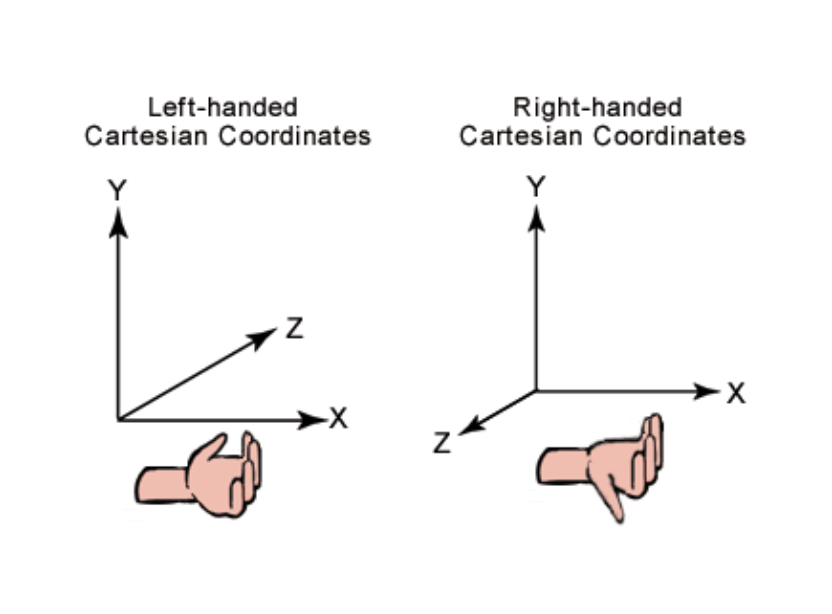
\includegraphics[width=0.7\columnwidth]{images/overview/left-right-hand.png}
  \end{figure}

  In left-handed system, positive Z extends into the screen. In right-handed
  system, positive z extends out of the screen.

  \begin{itemize}
    \item \textbf{Programmable systems does not enforce handedness}
    \begin{itemize}
      \item Metal, WebGL, DirectX all use left-handed system by default
    \end{itemize}
    \item Units do not have specific meanings
    \item Left, right handed coordinate systems only differ in the direction of
    positive z
    \item To convert between the two systems, simply negate the z-axis
  \end{itemize}
